\section{Comparación de Arquitecturas}

\subsection{Conociendo el estado actual}

Con la notación de las arquitecturas objetivo establecidas, al igual que el desarrollo del módulo encargado de la construcción y validación de los archivos de configuración; lo siguiente era la definición del proceso de la comparación entre la arquitectura actual y la arquitectura de referencia. Este proceso, nos permitirá evaluar el estado del sistema y, por consiguiente, establecer las acciones a tomar con el fin de adaptar la arquitectura hacia el estado objetivo establecido.

Esto requiere conocer el estado actual del sistema, al igual que el conocer el estado objetivo. Siendo así, y ya teniendo la posibilidad de declarar las necesidades de la aplicación, lo siguiente es establecer una manera de determinar el estado del sistema. Dado el enfoque hacia los datos recolectados, es necesario el precisar la manera en la que conoceríamos en qué estado se encuentra el sistema.

Partiendo de esto, lo primero era el identificar los puntos de acceso por los cuales podríamos acceder a los datos, en el caso de Smart Campus UIS, como se observa en la figura \ref{fig:ArquitecturaSmartCampus}, hay dos maneras en las que podemos acceder a los datos. La primera, es haciendo consultas a la base de datos en la cual se guardan los registros; la segunda, implica recibir los mensajes que viajan por el bus de datos, sea el de los adaptadores de descripción o el de los dispositivos con el servicio de mensajería , y procesar cada uno de los mensajes.

\begin{figure}[ht]
    \centering
    \caption{Arquitectura del prototipo de Smart Campus definido por }\citeA{msc_henry_2022}
    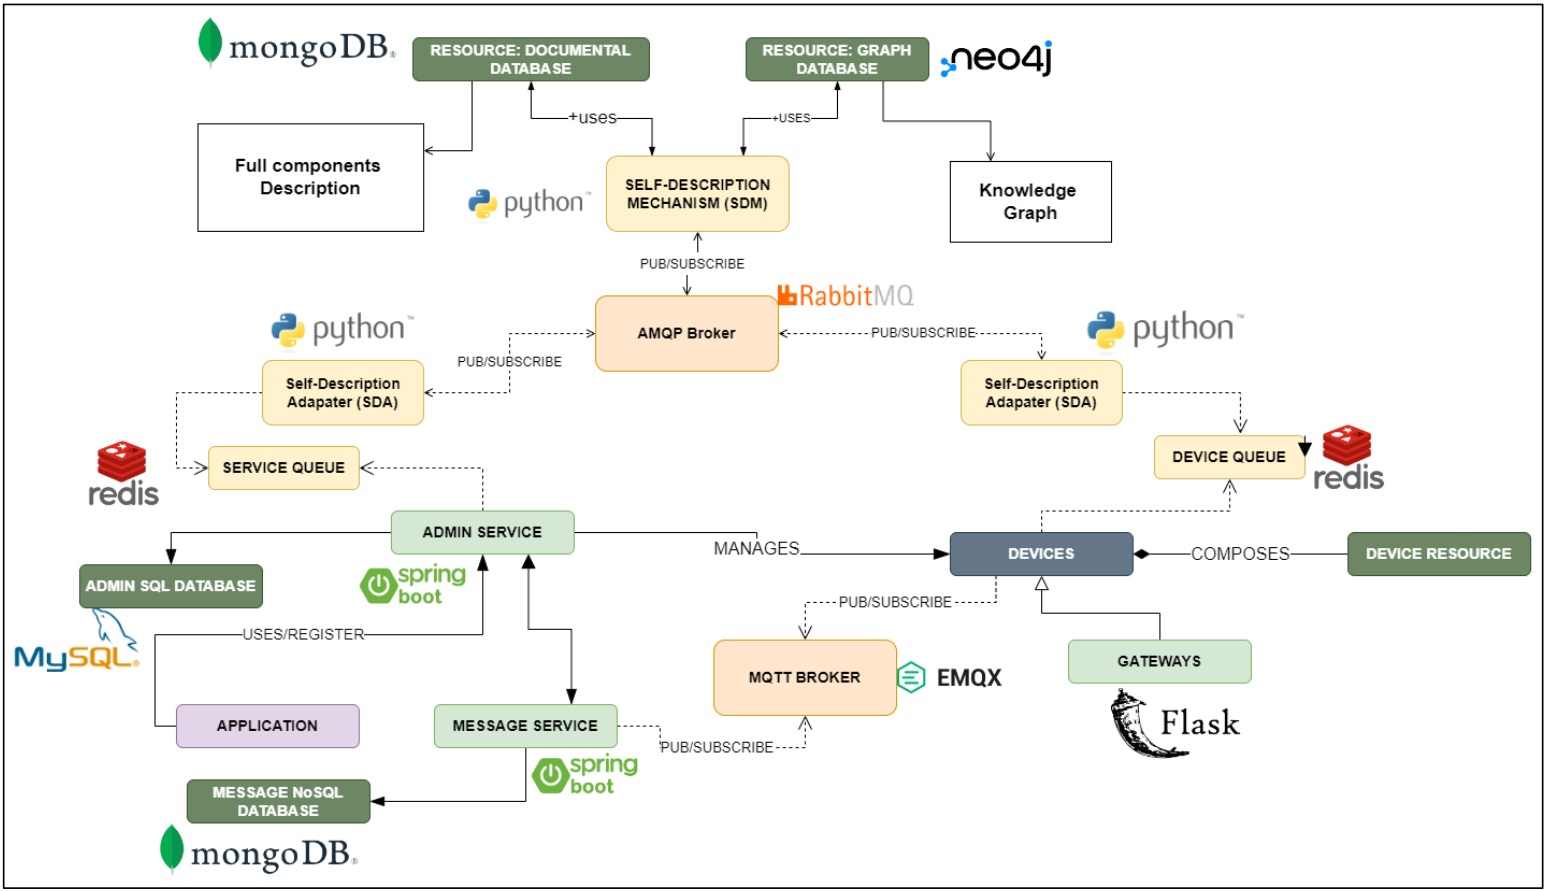
\includegraphics[width=\linewidth]{images/ArquitecturaSmartCampus.png}
    \label{fig:ArquitecturaSmartCampus}
\end{figure}

Ahora, cada una de las maneras de acceder a los datos es viable, y podría permitir la implementación correspondiente para determinar el estado del sistema. Sin embargo, de entre las tres opciones, se escogió el procesamiento de los mensajes de los adaptadores de descripción, enviados por AMQP. Esta decisión se debe a algunas de las ventajas que posee el protocolo sobre la consulta a base de datos. Entre estas destacan la menor latencia en la recuperación y la direccionalidad de datos, comparado con las consultas. 

La primera se refiere a la menor cantidad de saltos de servicios antes de que los datos sean guardados en la base de datos, lo que aumenta el tiempo en el que estos estarán disponibles, sumado a el tiempo ejecución de la consulta. Así mismo, la última refiriéndose a que el protocolo AMQP, gracias a su modelo pub/sub, permite el poder procesar los datos a medida que estos van llegando, y no en intervalos discretos de tiempo, lo cual podría afectar la toma de decisiones.

